\documentclass{beamer}
%
% Choose how your presentation looks.
%
% For more themes, color themes and font themes, see:
% http://deic.uab.es/~iblanes/beamer_gallery/index_by_theme.html
%
\mode<presentation>
{
  \usetheme{default}      % or try Darmstadt, Madrid, Warsaw, ...
  \usecolortheme{default} % or try albatross, beaver, crane, ...
  \usefonttheme{default}  % or try serif, structurebold, ...
  \setbeamertemplate{navigation symbols}{}
  \setbeamertemplate{caption}[numbered]
} 

\addtobeamertemplate{navigation symbols}{}{%
    \usebeamerfont{footline}%
    \usebeamercolor[fg]{footline}%
    \hspace{1em}%
    \insertframenumber/\inserttotalframenumber
}
\usepackage[english]{babel}
\usepackage[utf8x]{inputenc}

\title[Your Short Title]{Refresh Strategies for Continuous Active Learning}
\author{Nimesh Ghelani}
\institute{University of Waterloo}
\date{03 July 2018}

\begin{document}

\begin{frame}
  \titlepage
\end{frame}

% Uncomment these lines for an automatically generated outline.
%\begin{frame}{Outline}
%  \tableofcontents
%\end{frame}

% \section{Purpose}

% \begin{frame}{Purpose}
% \begin{itemize}
%     \item Discussion about my work in-progress
%     \item Get feedback and criticism
% \end{itemize}
% \end{frame}

\section{Background}
\begin{frame}{Background}
    Some problems:
    \begin{itemize}
        \item Legal eDiscovery
        \item Systematic Review
        \item Building test collection
    \end{itemize}

    \vskip 1cm
    The objective is to find as many relevant document as possible with minimal
    assessments costs

    \vskip 0.5cm
    High Recall problem
\end{frame}

\begin{frame}{Background - TAR}
    Technology Assisted Review (TAR): computer-assisted methods to do eDiscovery

    \vskip 1cm
    Continuous Active Learning (CAL):
    \begin{itemize}
        \item A TAR protocol
        \item Machine Learning to suggest likely-to-be-relevant documents for
            assessment
        \item Continuously incorporate relevance judgments to enhance the
            classifier
    \end{itemize}
\end{frame}

\begin{frame}{Background - Continuous Active Learning}
\begin{figure}
 \centering 
 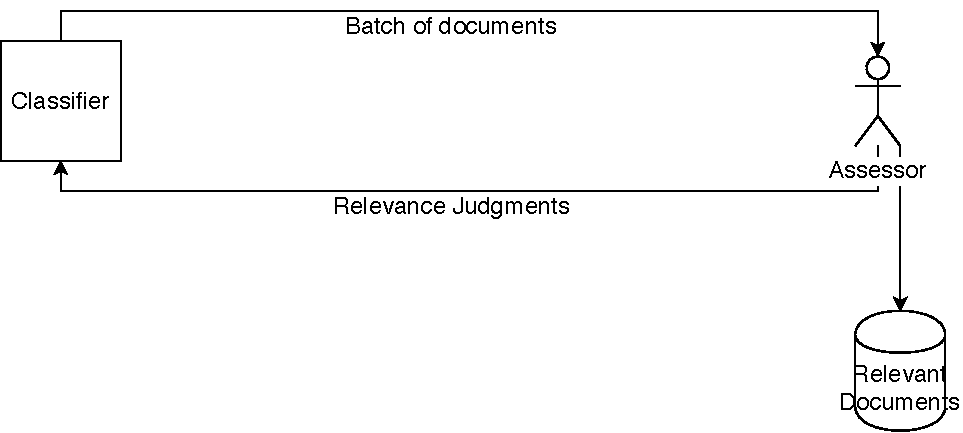
\includegraphics[width=1.0\textwidth]{diag.pdf}
 \caption{Simplified view of a CAL process}
\end{figure}
\end{frame}

\begin{frame}{Background - Refresh}
Refresh:
\begin{itemize}
    \item Use available judgments to build a classifier
    \item Produce next set of documents to be judged
    \item Computationally Expensive!
\end{itemize}

Refresh Strategy
\begin{itemize}
    \item When to refresh?
    \item How to refresh?
\end{itemize}
\end{frame}

\section{Objective}
\begin{frame}{Objective}
Investigate various refresh strategies; their effectiveness and efficiency.
\end{frame}


% \section{Outline}
% \begin{frame}{Outline}
% \begin{itemize}
%     \item Implementation
%     \item Dataset
%     \item Refresh Strategies
%     \begin{itemize}
%         \item Static batch sizes
%         \item Partial refresh
%         \item Precision based
%         \item Recency Weighting
%         \item Forgetting
%     \end{itemize}
%     \item Conclusion
%     \item Future Work
% \end{itemize}
% \end{frame}



% \section{Implementation}
% \begin{frame}{Implementation}
% \begin{itemize}
%     \item Implementation of BMI in C++
%     \begin{itemize}
%         \item Fast
%         \item Easy to use and configure (CLI/HTTP)
%         \item Extendable (components as abstractions  which can be replaced/modified easily)
%     \end{itemize}
%     \item Useful research tool
%     \item Used in
%     \begin{itemize}
%         \item TREC 2017 Core Track effort by UWatMDS
%         \item User Study and Demo (papers submitted to SIGIR 2018)
%     \end{itemize}
%     \item Operates entirely in-memory
%     \begin{itemize}
%         \item Requires all the documents in the memory (Drawback)
%     \end{itemize}
% \end{itemize}
% \end{frame}


\section{Refresh Strategies}

\begin{frame}{Refreshing in Original CAL (BMI)}
Train and score all documents every $k$ assessments ($k$ increases exponentially)

\vskip 1cm
After every refresh,
$k← k + (k + 9)/10$
\end{frame}


\subsection{Static Batch Sizes}
\begin{frame}{Static Batch Sizes}
Train and score all documents after every $k$ assessments ($k$ is static)
\vskip 1cm
$k = 1$
\begin{itemize}
\item Effective
\item High computation cost
\end{itemize}
\end{frame}


\begin{frame}
\begin{figure}
 \centering 
 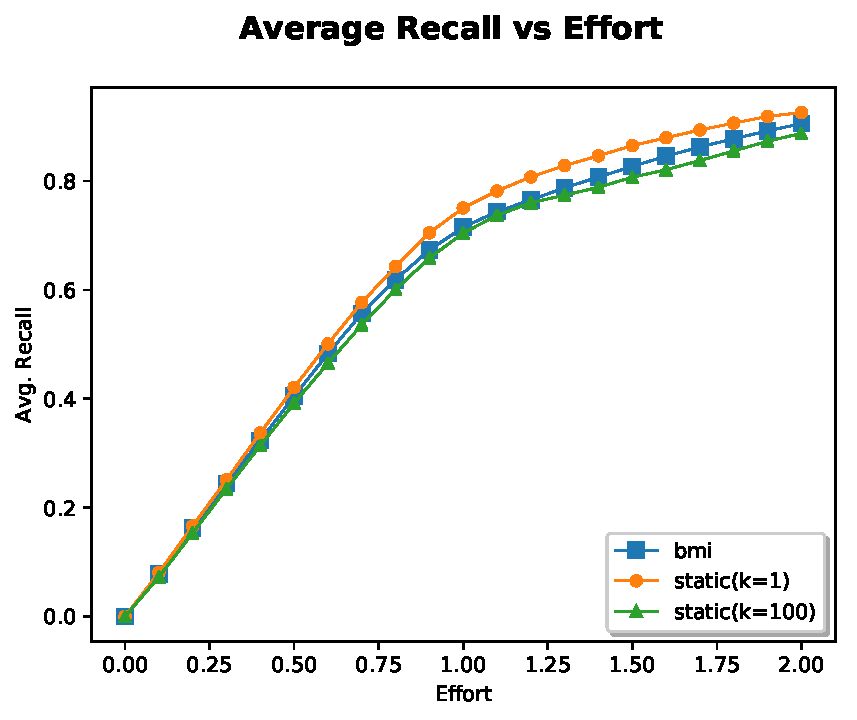
\includegraphics[width=1.0\textwidth]{static1.pdf}
\end{figure}
\end{frame}


\subsection{Partial Refresh}
\begin{frame}{Partial Refresh}
Perform frequent refreshing on a smaller set of data

Periodic complete refresh

\vskip 1cm
After every judgment:
\begin{itemize}
    \item train on all available judgments
    \item re-score high ranking documents from previous full refresh
\end{itemize}
 
Parameters
\begin{itemize}
    \item Size of partial re-score document set ($s$)
    \item Period for full refresh ($k$)
\end{itemize}

\end{frame}


% \begin{frame}{Partial Refresh}
% This strategy can help with the high memory costs
% \vskip 0.5cm
% Partial Refreshes are fast and performed on small set of data which can be stored in the memory

% \vskip 0.25cm
% Full Refresh can be performed in the background (reading from disk)
% \end{frame}


\begin{frame}
\begin{figure}
 \centering 
 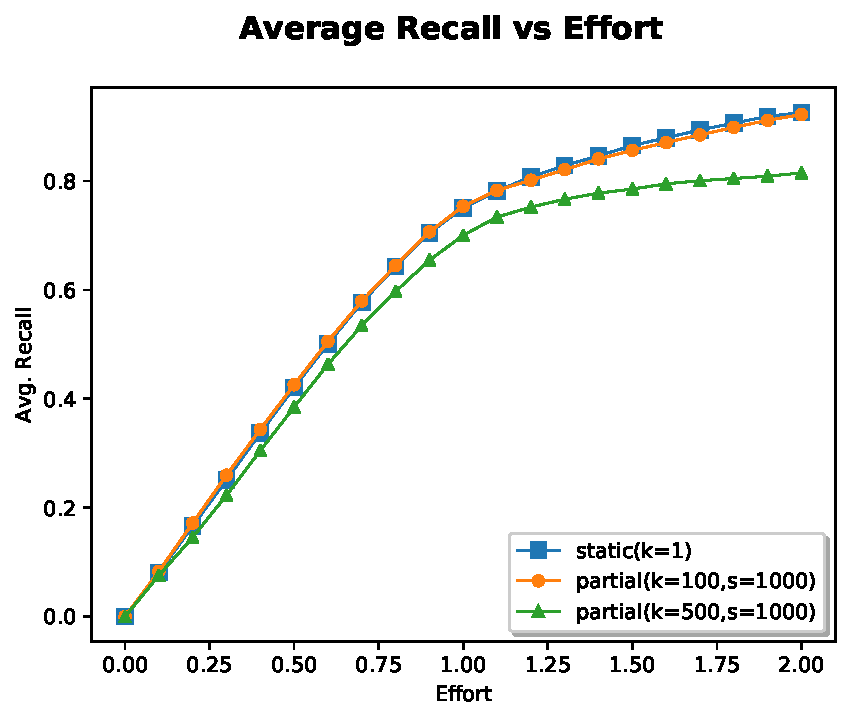
\includegraphics[width=1.0\textwidth]{partial1.pdf}
\end{figure}
Parameters
\begin{itemize}
    \item Size of partial re-score document set ($s$)
    \item Period for full refresh ($k$)
\end{itemize}
\end{frame}

\subsection{Precision Based Refreshing}
% Interesting because a good precision based strategy will give a better explanation on when to refresh
\begin{frame}{Precision Based Refreshing}
Refresh when ``output quality'' falls below some threshold
\vskip 1cm
\textbf{Problem:} Defining ``output quality''

\vskip 1cm
Refresh when the fraction of relevant judgments in the last $k$ judgments fall below $p$
\end{frame}


\begin{frame}
\begin{figure}
 \centering 
 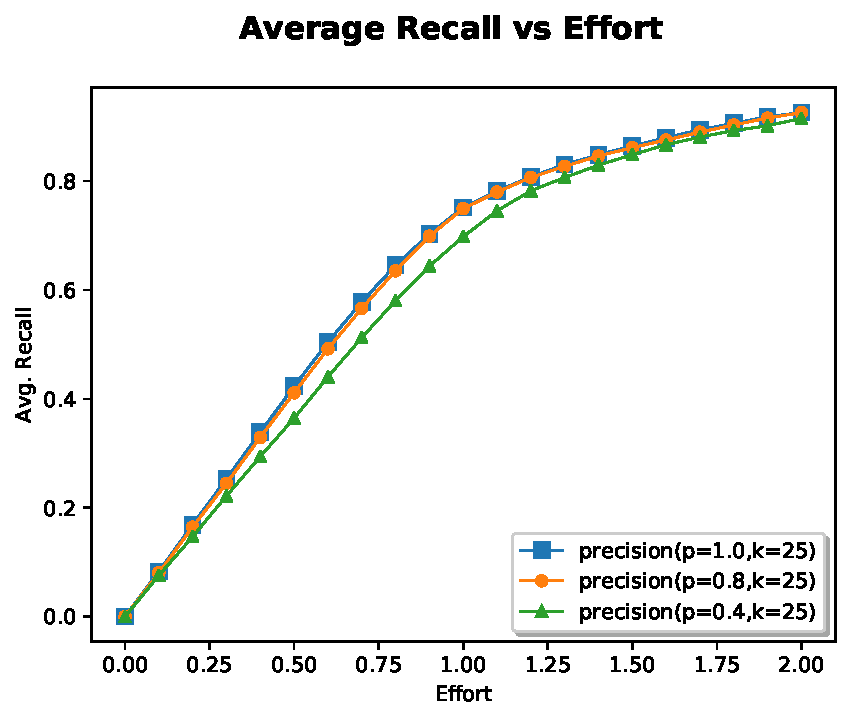
\includegraphics[width=1.0\textwidth]{prec1.pdf}
\end{figure}
\end{frame}

\begin{frame}
\begin{figure}
 \centering 
 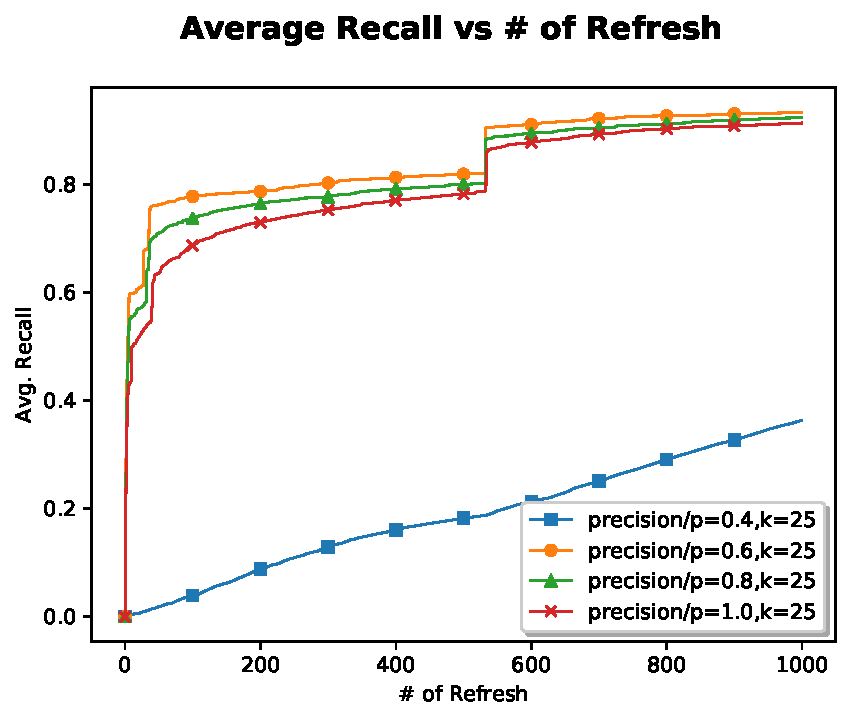
\includegraphics[width=1.0\textwidth]{prec2.pdf}
\end{figure}
\end{frame}


\subsection{Recency Weighting}
\begin{frame}{Recency Weighting}
Recent judgments ``weighted'' more in training
\vskip 1cm

\textbf{Default training:} loss computed based on a random positive and a negative judgment (numerous iterations)

\vskip 0.5cm
\textbf{Modified training:} modify sampling such that latest judgment is $k$ times more likely to be selected than the first judgment (fit a linear curve).
\end{frame}


\begin{frame}{Recency Weighting}
With original settings, recency weighting didn't result in any difference

\vskip 1cm
\textbf{Possible Reason:} Very high number of training iterations ($it = 10^5$)
\end{frame}


\begin{frame}
\begin{figure}
 \centering 
 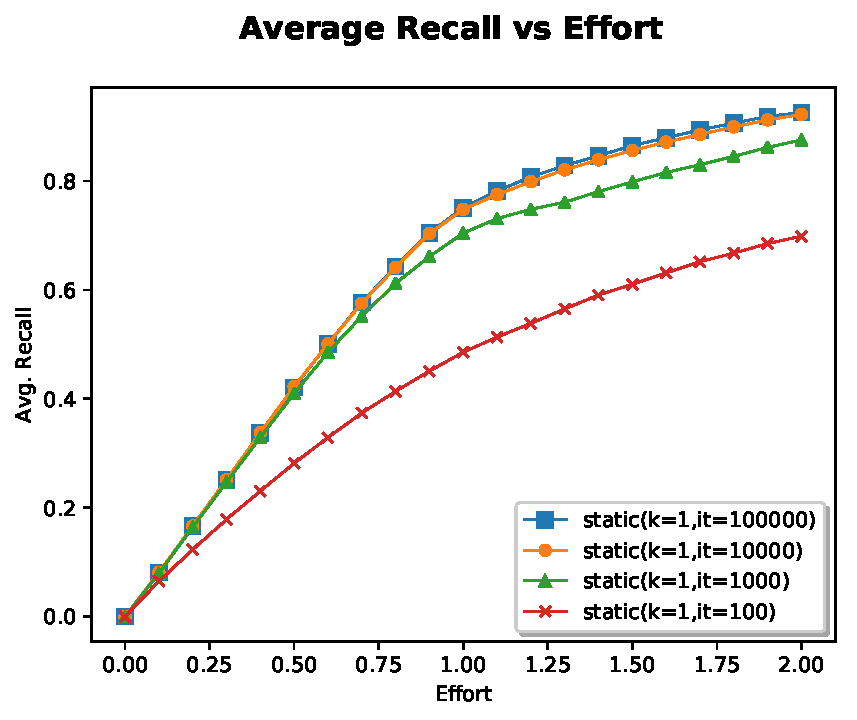
\includegraphics[width=1.0\textwidth]{train1.pdf}
\end{figure}
\end{frame}

\begin{frame}
\begin{figure}
 \centering 
 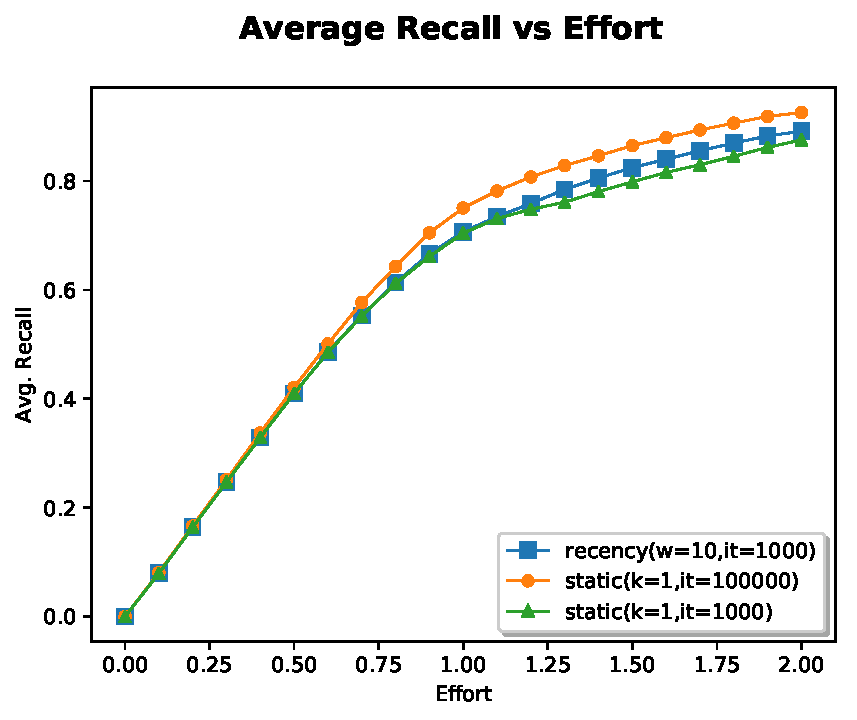
\includegraphics[width=1.0\textwidth]{rec1.pdf}
\end{figure}
\end{frame}

\section{Conclusion}
\begin{frame}{Conclusion/Summary}
\begin{itemize}
    \item Frequent refreshing helps achieving higher recall using lesser
       assessment effort
    \item Static batch size of 1 performs great but is computationally expensive
        \begin{itemize}
            \item With an efficient implementation, practical for most datasets and hardware
            \item Various alternative strategies can achieve similar performance while
            being computationally efficient
        \end{itemize}
\end{itemize}
\end{frame}

\end{document}

